\chapter{ANN模型结构}
\par
目前,目标检测中two-stage系列模型基本采用以下的流程:假设物体边框,对每个边框内进行特征再采样,最后使用分类器进行分类。
这个流程比较流行,但它们存在一个问题:虽然检测效果都很好,但是这些方法对于设备来说计算量过大,甚至需要高端硬件的支持,
对于实时系统来说太慢。最快的检测器也没有到我们理想的速度。考虑后续作为SNN转化的基础模型,我们选择速度较快的单阶段检测器。
\par
下面先介绍SSD算法---多类别单阶段检测器。SSD的设计为端到端训练,精度高,甚至在低分辨率的图像上效果也不错。
其设计理念可总结为:
(1)采用多尺度特征图用于检测(较大的特征图检测小目标,小的特征图检测大目标)
(2)采用卷积进行检测
(3)设置先验框(减小训练难度)。
下面对网络结构进行详细介绍
\section{SSD}
\subsection{基础网络}
\par
我们首先放出SSD的网络结构,如下图\mycite{2016SSD}所示:
\begin{figure}[htbp]
	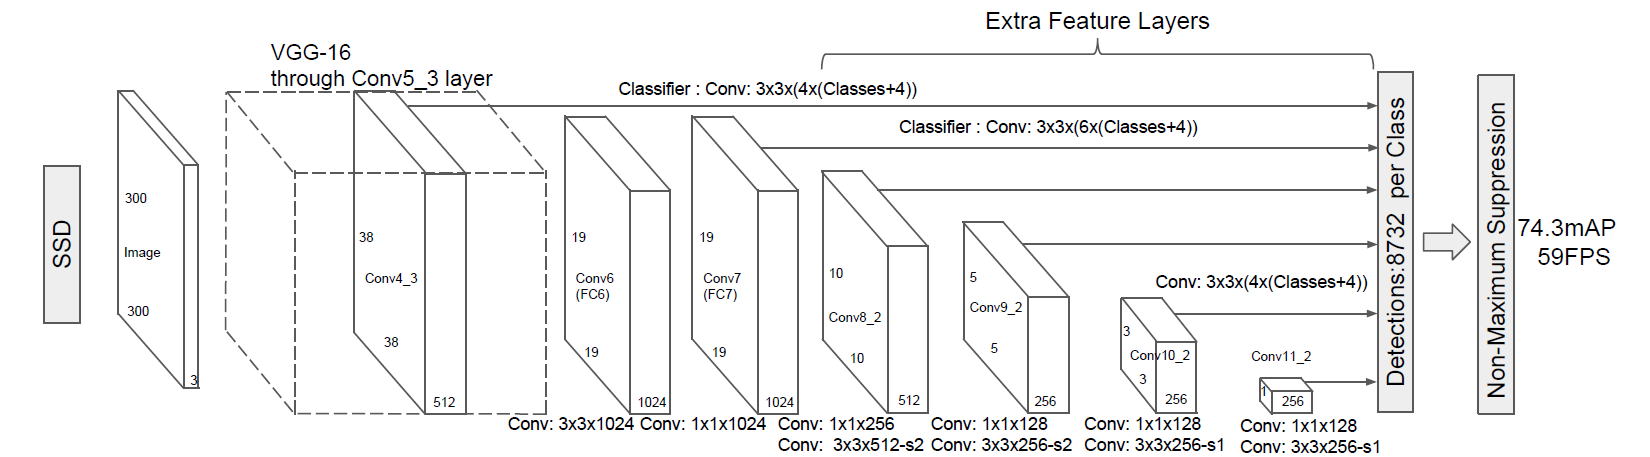
\includegraphics[width=1\textwidth]{figures/ssdnet.png}
	\setlength{\abovecaptionskip}{0cm}  
	\setlength{\belowcaptionskip}{0cm}  
	\caption{ssd网络结构}
\end{figure}
\par
可以看到原始的SSD网络是以VGG-16作骨干网络(Backbone)的,SSD从六个卷积层上提取信息,所用到的特征图以及大小如下表所示:
\par
{
\begin{center}
\begin{tabular}{|rr|}
	\hline
	feature map & 大小\\
	\hline
	Conv4\_3 & 38*38\\
	Conv7 & 19*19\\
	Conv8\_2 & 10*10\\
	Conv9\_2 & 5*5\\
	Conv10\_2 & 3*3\\
	Conv11\_2 & 1*1\\
	\hline
\end{tabular}
\end{center}
}
\par
SSD一共有6层多尺度提取的网络,每层分别对 loc 和 conf进行卷积,得到相应的输出。以conv4\_3为例:
\begin{figure}[!ht]
	\centering
	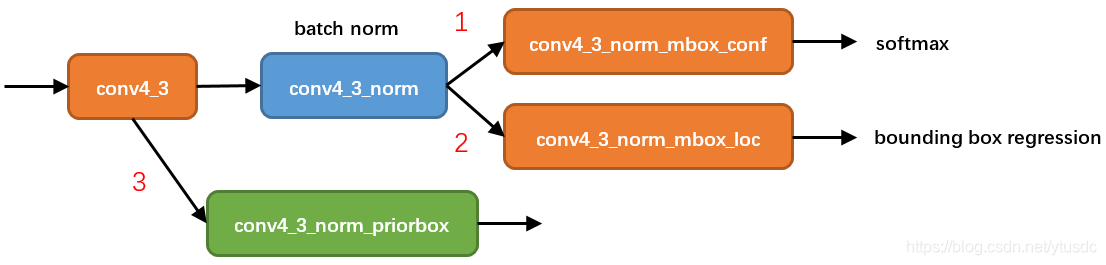
\includegraphics[width=1\textwidth]{figures/conv43.png}
	\caption{单个特征层的特征提取}
\end{figure}
\par
经过conv4\_3层之后,网络分为了3条路线:一是用于softmax分类目标和背景,计算置信度的特征层;二是用于边界框预测的回归层;
三是用于生成并保留先验框位置信息。目标检测中的分类加定位,就是分别由分类层和回归层实现。其中一个细节是这里只有conv4\_3层
进行了Normalization操作,原因是该层特征图大小是$38 \times 38$,该层比较靠前,为了保证和后面的检测层差异不大,
就在后面加了L2 Normalization层。
\par
但不是每一层都计算softmax和regression,这样计算量大,实际需要多个featuremap协作,也就是把所有特征层的关于类别或者位置的特征连接起来,再进行softmax和
bounding box预测。
\begin{figure}[H]
	\centering
	\setlength{\abovecaptionskip}{-1cm}  
	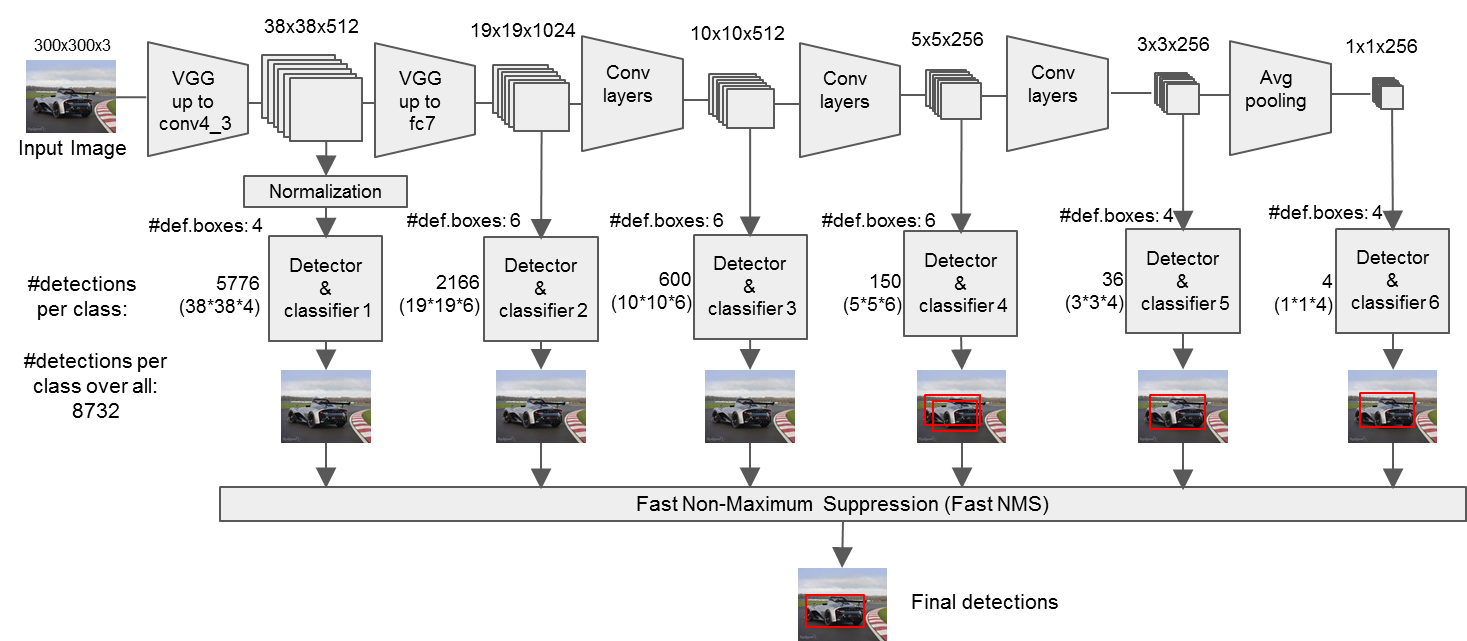
\includegraphics[width=1\textwidth]{figures/liucheng.png}
	\caption{多个特征层的协作}
\end{figure}
\subsection{先验框}
\par
SSD之所以提升了推理速度,很大一部分原因是其放弃了以前在原图上进行区域提议(region proposal)的操作,
SSD直接生成一系列先验框(default box),以先验框为初始的box,计算其与正确标注框(gound truth)的相对坐标,
之后对相对坐标进行编码,根据先验框位置再解码就可得到GT框。整个过程通过网络的一次前向传播即可完成。
在特征图上生成的先验框如下图\mycite{2016SSD}所示:
\begin{figure}[H]
	\centering
	\setlength{\abovecaptionskip}{0cm}  
	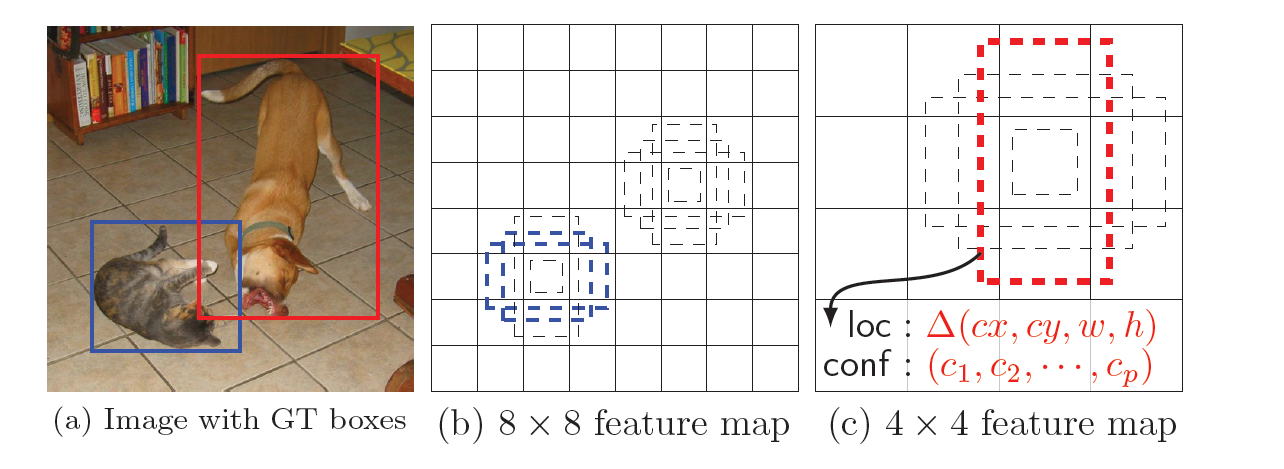
\includegraphics[scale=0.45]{figures/SSD.png}
	\caption{SSD的先验框}
\end{figure}
生成规则在\mycitex{2016SSD}中给出了具体的公式,此处不再提及。
\subsection{损失函数}
\par
SSD的损失函数包含两个部分,一个是定位损失$L_{loc}$,一个是分类损失$L_{conf}$,整个损失函数表达如下:
\[
L(x,c,l,g)=\frac{1}{N}(L_{conf}(x,c)+\alpha L_{loc}(x,l,g))
\]
\par
其中$N$是先验框正样本数量,$c$是类别置信度预测值,$l$是先验框对应的边界框预测值,$g$是ground truth的位置参数,
$x$代表网络的预测值。
\par
对于位置损失,采用Smooth L1 Loss,
位置信息都是encode之后的数值。而对于分类损失,
首先需要使用hard negtive mining将正负样本按照1:3 的比例把负样本抽样出来,
抽样的方法是:针对所有batch的confidence,按照置信度误差进行降序排列,
取出前top\_k个负样本。

\section{YOLO}
\par
接着介绍YOLO模型,其全称是You Only Look Once: Unified, Real-Time Object Detection,这也表明了Yolo算法的特点:只需要一次CNN运算,进行的是端到端的统一预测。YOLO有很多实现版本,这里以Yolo-v1\mycite{YOLO}为例,进行模型结构介绍。
\subsection{网络结构}
\par
Yolo网络结构,如下图\mycite{YOLO}所示:
\begin{figure}[H]
	\centering
	\setlength{\abovecaptionskip}{0cm}  
	\setlength{\belowcaptionskip}{0cm}  
	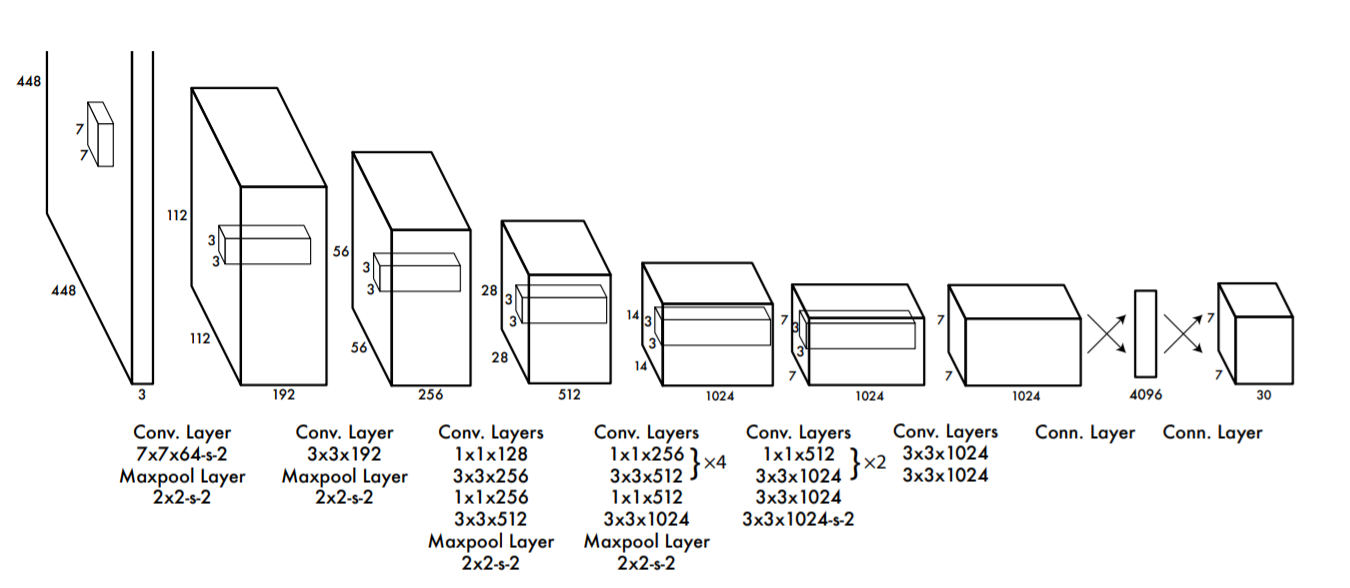
\includegraphics[width=1\textwidth]{figures/yolonet.png}
	\caption{Yolo网络结构}
\end{figure}
\par
可以看到,Yolo采用卷积网络来提取特征,然后使用全连接层来得到预测概率和坐标。网络结构中包含24个卷积层和2个全连接层。
其中卷积层,主要使用1x1卷积进行通道降维,然后紧跟3x3卷积提取特征。
对于卷积层和全连接层,不使用常见的ReLu激活函数,而是采用Leaky ReLU激活函数:$max(x,0.1x)$,但需要注意的是最终层仍使用线性激活函数ReLu。
\subsection{损失函数}
\par
类似地,检测在Yolo中也是回归问题,采用的是均方差损失函数。
整个算法的损失是由预测框的坐标误差,有无包含物体的置信度误差以及网格预测类别的误差三部分组成,三部分的损失都使用了均方误差的方式来实现。
具体表示如下:
\begin{equation}
	\begin{array}{l}
	\lambda_{\text {coord }} \sum_{i=0}^{S^{2}} \sum_{j=0}^{B} \mathbb{1}_{i j}^{\text {obj }}\left[\left(x_{i}-\hat{x}_{i}\right)^{2}+\left(y_{i}-\hat{y}_{i}\right)^{2}\right] \\
	\quad+\lambda_{\text {coord }} \sum_{i=0}^{S^{2}} \sum_{j=0}^{B} \mathbb{1}_{i j}^{\text {obj }}\left[\left(\sqrt{w_{i}}-\sqrt{\hat{w}_{i}}\right)^{2}+\left(\sqrt{h_{i}}-\sqrt{\hat{h}_{i}}\right)^{2}\right] \\
	+\sum_{i=0}^{S^{2}} \sum_{j=0}^{B} \mathbb{1}_{i j}^{\text {obj }}\left(C_{i}-\hat{C}_{i}\right)^{2} \\
	+\lambda_{\text {noobj }} \sum_{i=0}^{S^{2}} \sum_{j=0}^{B} \mathbb{1}_{i j}^{\text {noobj }}\left(C_{i}-\hat{C}_{i}\right)^{2} \\
	+\sum_{i=0}^{S^{2}} \mathbb{1}_{i}^{\text {obj }} \sum_{c \in \text { classes }}\left(p_{i}(c)-\hat{p}_{i}(c)\right)^{2}
	\end{array}
	\end{equation}
对于定位误差,采用较大的权重$\lambda_{coord}=5$。然后其区分不包含目标的边界框与含有目标的边界框的置信度.
对于前者,采用较小的权重值$\lambda_{noobj}=0.5$。其它权重值均设为1。对中心点直接进行均方误差,对宽高则使用平方根进行误差计算。
进行平方根均方误差的原因是较小的边界框中,定位误差要比较大的边界框要更敏感,为了区分这种不对等情况,所以对定位损失中的宽高损失加上了平方根。
\subsection{预测部分}
\par
以预测推理一张图片为例,Yolo输入图像后,输出7x7x30维度的张量,
即:将图片以物体中心点位置划分为7x7,每个单元格独立检测。
物体的中心落在哪个单元格,就由那个单元格负责预测。如下图\mycite{YOLO}所示:
\begin{figure}[H]
	\centering
	\setlength{\abovecaptionskip}{0cm}  
	\setlength{\belowcaptionskip}{0cm}  
	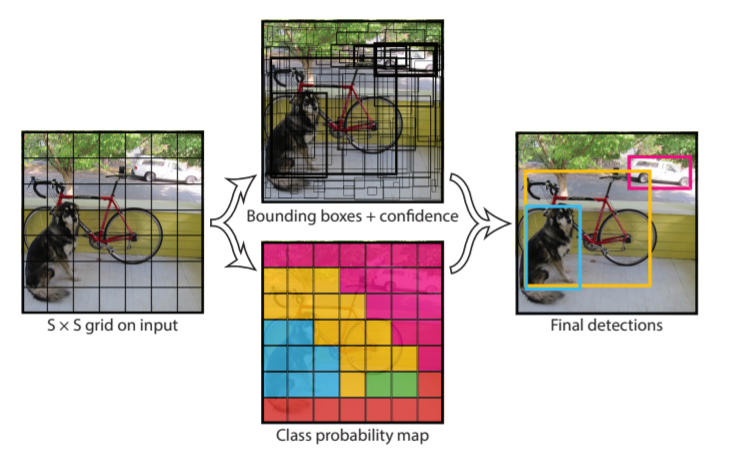
\includegraphics[width=1\textwidth]{figures/yologrid.png}
	\caption{Yolo检测方式}
\end{figure}
\par
最后张量维度为30,由(2*5+20)构成,其中2:每个单元格预测数量,5:$(x,y,w,h,score)$,20:模型可以预测20个种类。